% Editable report section: Source and Reproduction Materials
\section{Source and Reproduction Materials}
\label{sec:a}

The complete source is supplied under \path{02_SourceCode/src/fortune} in the review package, with a companion searchable plain-text source listing in \path{01_Report/source_listing.txt}. The pytest suite is under \path{tests/}. The editable LaTeX report includes separate section files, a shared preamble and a BibTeX database. The PDF build script is included. Figures are reproduced by \path{tools/make_figures.py} from the program and recorded benchmark data.

\begin{figure}[!htbp]
\centering
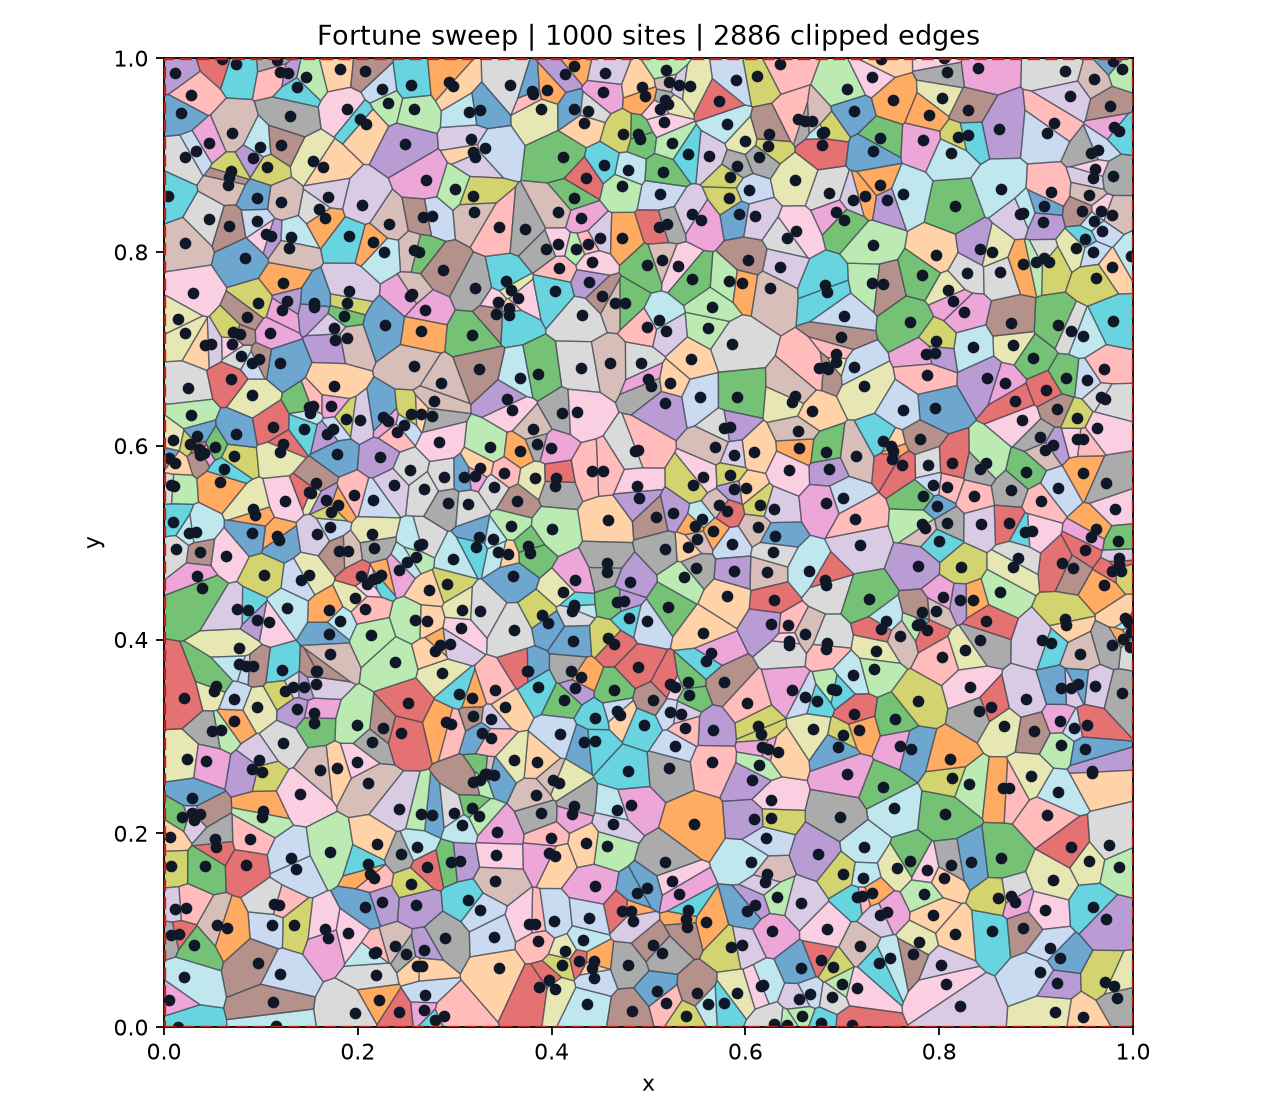
\includegraphics[width=0.90\linewidth,height=0.48\textheight,keepaspectratio]{large.png}
\caption{A 1,000-site diagram with labels hidden to preserve legibility.}
\label{fig:8}
\end{figure}

This dense example uses seed 2026 and the unit square. Labels are intentionally hidden for this preview; the CLI displays them by default. Construction statistics and machine-readable output remain independent of the drawing density.

The ZIP's isolated installation passed 139 tests; all eighteen loaded Fortune modules came from site-packages. Installed Canvas assets and Windows-launcher exports were verified. Logs and payload hashes are retained in \path{evidence/package-verification.json}.
